\begin{frame}{Постановка задачи} \hypertarget{slide\insertframenumber}{}
	Рассматривается объект управления
	\begin{align}
		\label{8}
		\dot x(t) &= Ax(t) + B(t)\redcolor{u(t)},\\
		\label{9}
		y(t) &= C^\top x(t),
	\end{align}
	где  $x(t)\in\rea^k$,  $y\left( t \right) \in \rea^m$,  $u\left( t \right) \in\rea^\ell $, \par 
	\vspace{4mm}
	$B(t)=B(\xi(t))$ --- матрица входов с переменными параметрами
	\begin{align}	\label{10}
		B(t) &= B_0 \,  \xi^\top (t) H,\\
		\label{11}
		\dot \xi(t) &=\Gamma \xi(t)+G\redcolor{u(t)},
	\end{align}
	где $\xi(t) \in \rea^n$, \redcolor{$\xi(0)$} --- неизвестны, матрицы $ \Gamma, G$, $ B_0 \in \rea^k$, $H\in\rea^{n \times \ell}$ --- известны.
	
	\vspace{4mm}
	
	Требуется синтезировать закон управления $u(t)$, обеспечивающий ограниченность всех переменных состояния и выполнение целевого условия
	\begin{align}\label{12}
		\mathop {\lim }\limits_{t \to \infty } \left( {y(t)  - y^*(t)} \right) = 0.
	\end{align}
	
\end{frame}

\begin{frame}\frametitle{Синтез закона управления по выходу}
	\small %\scriptsize %\footnotesize %
	\begin{statement} \label{st2}
		Закон управления вида 
		\begin{align}\label{16}
			u(t) &= H^\top \xi_d V(t) +K_1^\top \redcolor{\xi(t)}, \\ 
			\dot \xi_d(t) &= (\Gamma +GK_1^\top)\xi_d(t) + GH^\top \xi_d(t)V(t), \\  
			V(t) &=  (\xi_d^\top(t) HH^\top \xi_d(t))^{-1} (\bluecolor{\tau(t)} - \xi_d^\top(t) HK_1^\top \xi_d(t)),
		\end{align}
		где начальные условия  $\xi_d(0)$ выбраны так, что $\|\xi_d(t)\|\in {\cal L}_\infty$ и $H^\top \xi_d(t) \neq 0$, с входным сигналом
		\begin{align}
			\bluecolor{\tau(t)} &= K_2^ \top \left( {\hat x\left( t \right) - {x^*}\left( t \right)} \right) + h_y^ \top \Gamma _y^k{\xi _y}\left( t \right),\\  \label{20}
			\dot{\hat x}\left( t \right) &= A\hat x\left( t \right) + B_0 \tau \left( t \right) + L\left(y(t) - C^\top \hat x(t)\right),
		\end{align}
		где	${x^*}\left( t \right) = \left[ {\begin{array}{*{20}{c}}
				{h_y^ \top } \\ 
				\vdots  \\ 
				{h_y^ \top \Gamma _y^{k - 1}} 
		\end{array}} \right]{\xi _y}\left( t \right)$, обеспечивает ограниченность всех переменных состояния и выполнение цели 
	\end{statement}	
\end{frame}


\begin{frame}{Оценка переменной $\xi(t)$}
	\hypertarget{slide\insertframenumber}{}
	%\small
	Продифференцируем \eqref{9} $k$ раз, перепишем в матричном виде, выразим вектор переменных $x(t)$ и подставим в уравнение $y^{(k)}(t)$. 
	\begin{align}\label{22}
		y^{(k)}= C^\top A^k \, W_y^{-1} \left( \varphi - F_1(u)\bluecolor{\xi} -F_2(u) \right) + C^\top A^{k-1}B_0 u^\top H^\top \bluecolor{\xi} + \ldots + {C^\top}{B_0}{\left( {\frac{d}{{dt}}} \right)^{k-2}}\left[ u^\top H^\top Gu \right].
	\end{align}
	
	Для исключения в выражении \eqref{22} неизмеряемой функции $\xi(t)$ воспользуемся методом GPEBO и рассмотрим фильтры вида
	\begin{align} \label{2.sigma1.ru}
		\dot \sigma_1 &= \Gamma \sigma_1 + Gu, \; \sigma_1(0)=0, \\
		\label{2.sigma2.ru}
		\dot \sigma_2 &= \Gamma \sigma_2, \qquad \sigma_2(0) =I.
	\end{align}
	Заметим, что для невязки $\tilde \xi(t) = \xi(t) - \sigma_1(t)$ имеем соотношение
	\begin{align*}
		\dot {\tilde {\xi}}(t)  = \Gamma \tilde \xi(t), \qquad
		\tilde \xi(0) =\xi(0),
	\end{align*}
	и $\tilde \xi(t)= \sigma_2(t)\xi(0)$. 
\end{frame}


\begin{frame}{Пример численного моделирования  1} \hypertarget{slide\insertframenumber}{}
	\begin{figure}[!h]
		\begin{subfigure}[t]{0.45\textwidth}
			\centering
			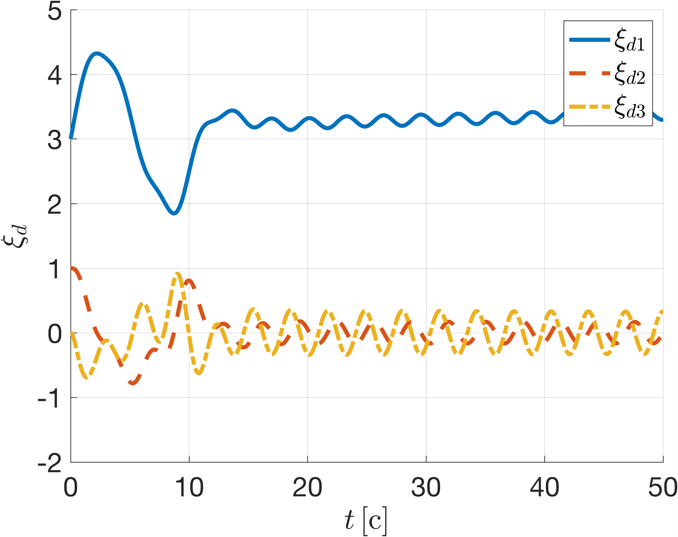
\includegraphics[width=0.5\linewidth]{figures/3.1xid.png}
			\caption{Временная диаграмма  $\xi_d$.}
		\end{subfigure}
		\begin{subfigure}[t]{0.45\textwidth}
			\centering
			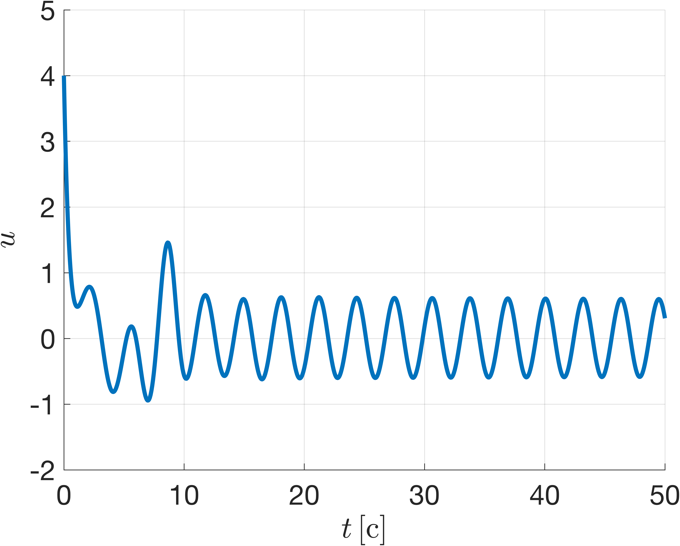
\includegraphics[width=0.5\linewidth]{figures/3.1u.png}
			\caption{Сигнал управления $u(t)$.}
		\end{subfigure}
		\begin{subfigure}[t]{0.45\textwidth}
			\centering
			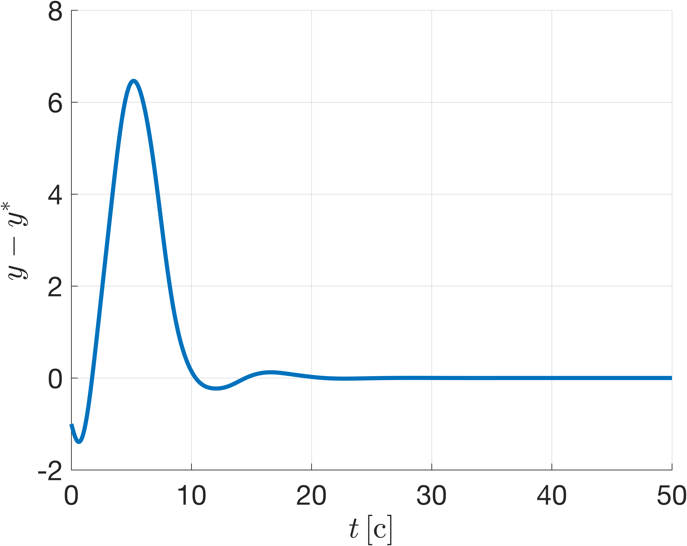
\includegraphics[width=0.5\linewidth]{figures/3.1ey.png}
			\caption{Ошибка регулирования $e(t)=y-y^*$.}
		\end{subfigure}
		\begin{subfigure}[t]{0.45\textwidth}
			\centering
			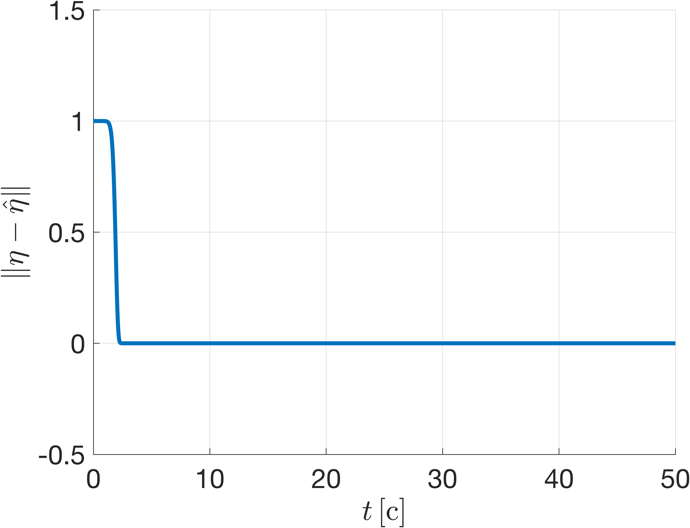
\includegraphics[width=0.5\linewidth]{figures/3.1eeta.png}
			\caption{Ошибка оценивания $\eta = \tilde \xi(0)$.}
		\end{subfigure}
		\label{f1}
	\end{figure}
\end{frame}